\section{Introduction}
Recent advances in reinforcement learning from verifiable rewards (RLVR) for large language models (LLMs) are increasingly shifting from single-turn to multi-turn agentic tasks~\citep{guo2025deepseek, hu2025openreasonerzero, cao2025skyrl, luo2025deepswe, gao2025beyond}.
Unlike single-turn tasks, multi-turn agentic tasks typically involves interacting with external environments, such as code repositories~\citep{jimenez2023swe}, web-browser~\citep{zhou2023webarena}, or even full computer operating systems~\citep{xie2024osworld} via iterative tool use. As a result, they often produce trajectories that often span dozens of turns and tens of thousands of tokens.

Training such agents with RL requires repeatedly rolling out policies in these environments and using the resulting trajectories for optimization. As task scale and complexity grow, rollout generation becomes a major bottleneck due to the heterogeneous environments and non-instantaneous feedback inherent in agentic tasks. 
For example, a single rollout in software engineering tasks often involves many sequential environment interactions, each of which may incur highly variable latency depending on the execution result or environment response.
In response, a number of agentic RL training frameworks have recently emerged~\citep{cao2025skyrlagent,jiang2025verltool,tan2025rllm,sheng2025verl,luo2025agentlightning,liu2025gem, xi2026agentgymrl}.

A counterintuitive design in existing frameworks is the tightly coupling agentic rollout with the RL training stack, with agent lifecycle handled within the trainer. This couples two modules with fundamentally different responsibilities leads to two major limitations.
\begin{enumerate}
    \item \textbf{Conflicting system requirements:} Rollout and policy training have fundamentally different resource and operational characteristics. Rollout is I/O-intensive, involving sandbox creation, long-lived tool sessions, and asynchronous coordination across hundreds of concurrent instances. Training, by contrast, is GPU-intensive, centered on forward and backward passes, and gradient synchronization. Coupling these workloads causes interference and reduces overall resource efficiency.
    \item \textbf{Difficult to migrate and maintain:} When rollout logic is embedded in RL trainer, migrating to a different training backend often requires re-implementing the entire agent execution pipeline. Likewise, improving the rollout infrastructure, such as supporting new runtime environments or tasks, often requires changes that propagate into the training codebase. In practice, this tight coupling slows progress on both fronts, as it makes independent experimentation and optimization on either side more difficult.
\end{enumerate}
These issues are likely to be further exacerbated by the growing need for rapid infrastructure iteration and more effective use of compute resources. If rollout and training are not decoupled from the begining, the accumulated system complexity can become a serious obstacle to scalability and long-term maintainability.

Drawing inspiration from the inference-as-a-service philosophy adopted by common LLM inference engines~\citep{kwon2025vllm, zheng2024sglang}, we adopt \texttt{rollout-as-a-service} as the core design principle for agentic RL training frameworks, decoupling the trainer from agentic rollout by treating the agentic rollout lifecycle as an independent service. 
We present \prorlagent, an open-source scalable infrastructure for multi-turn agentic rollout in RL training. 
Instead of implementing rollout as an in-process component of the RL trainer, \prorlagent serves the full rollout pipeline, from environment initialization to outcome evaluation, through an HTTP server. 
This design allows RL trainers to submit task instances and retrieve completed trajectories without managing any part of the rollout lifecycle. 
On one hand, this decoupled design allows rollout and training to run on different machines, separating I/O-intensive execution from GPU-intensive optimization; on the other hand, it improves extensibility and maintainability by decoupling rollout infrastructure from training backends.

In addition, \prorlagent provides several other features that support effective RL training for multi-turn agents. 
First, it adopts token-in/token-out communication throughout the training pipeline, allowing trainers to directly consume token-level trajectories while avoiding re-tokenization drift~\citep{team2025notokenization}. This makes training more stable and faithful to the original model outputs.
Second, \prorlagent provides extensible sandbox environments for agent execution, with flexible support for diverse tools and task. This makes it simple to host heterogeneous agentic tasks within a unified rollout service.
Third, \prorlagent is designed for rootless deployment in shared cluster environments. This makes it practical to run large-scale agentic rollouts under the permission and isolation constraints common in HPC settings.

\begin{figure}[t]
  \centering
  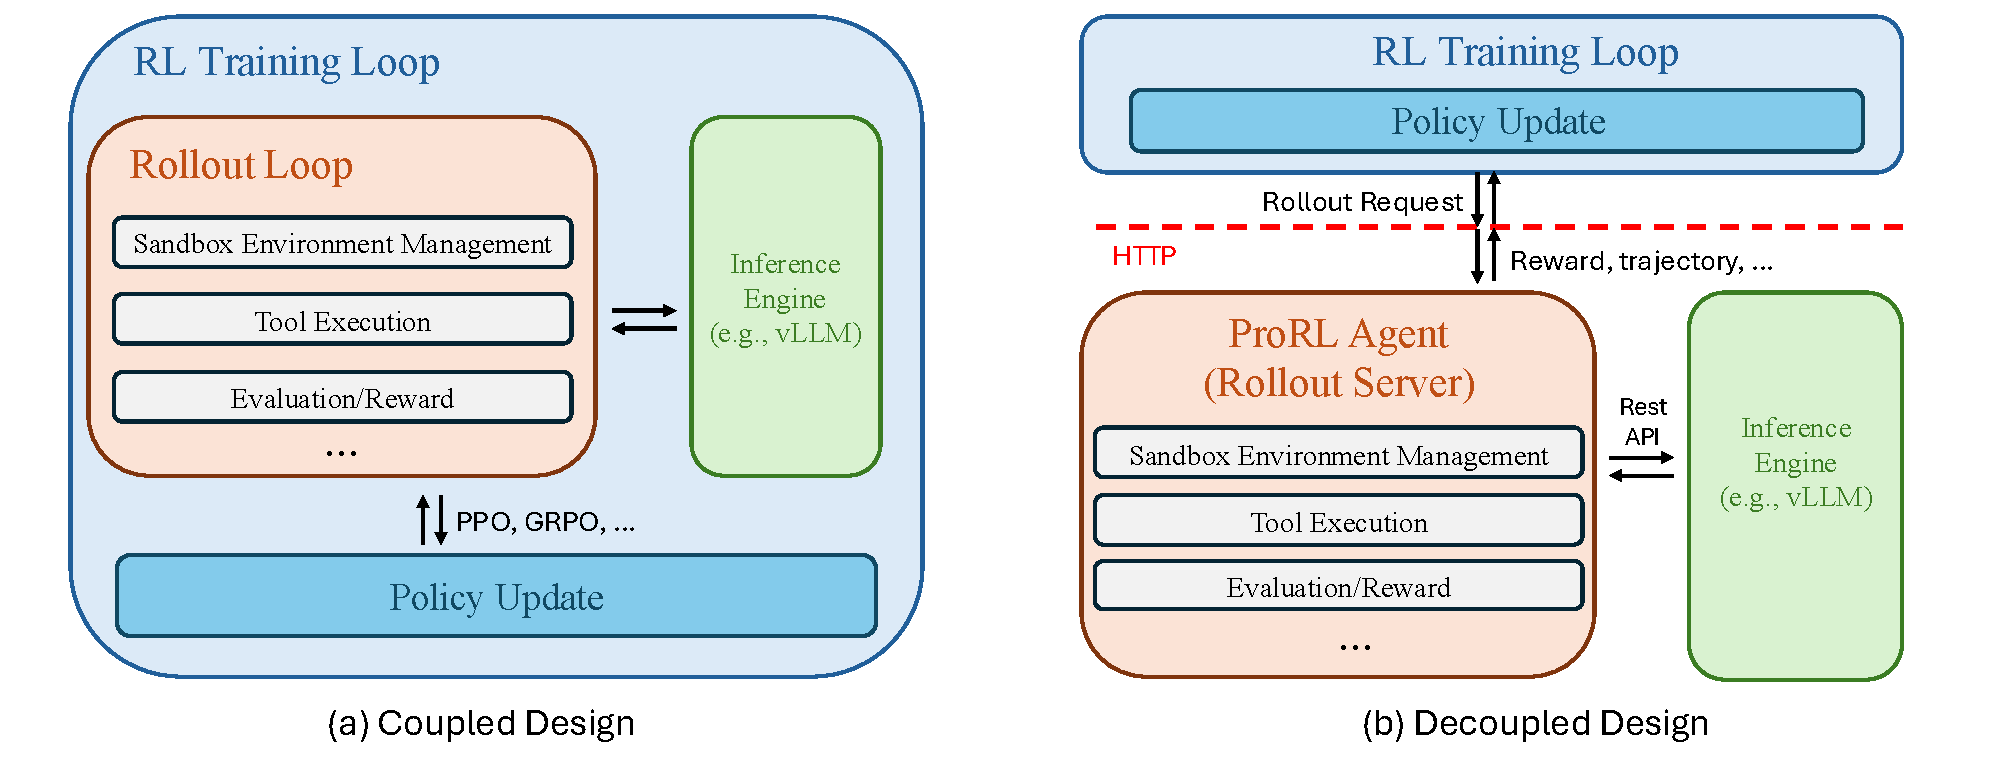
\includegraphics[width=1.0\linewidth]{figures/prorl_agent_decoupled.pdf}
\caption{\textbf{Coupled vs.\ decoupled designs.}
\textbf{Left:} Existing frameworks often embed the full agentic rollout lifecycle inside the RL training stack. 
\textbf{Right:} \prorlagent treats rollout as an independent HTTP service. The trainer submits rollout requests and receives completed trajectories and rewards, while the rollout server handles environment execution, tool use, evaluation, and inference coordination. This decoupled design improves resource isolation, portability, and extensibility.}
  \label{fig:decoupling}
  \label{fig:teaser}
\end{figure}

We validate \prorlagent by integrating it with ProRL training framework~\citep{prorl2025} for end-to-end RL training on software engineering tasks. Across 4B, 8B, and 14B model scales, it yields strong gains on SWE-Bench Verified. It also performs well in other agentic domains, including MATH, STEM, and coding. ProRL Agent is also integrated as part of NVIDIA NeMo Gym~\citep{nemo-gym}.

In summary, the main contributions of this work are:
\begin{itemize}
    \item We identify the key limitation in existing agentic RL training frameworks: multi-turn agentic rollout is typically tightly coupled with the RL training stack, even though rollout and training have fundamentally different resource and execution characteristics. To address this, we introduce ProRL Agent, an open-source and scalable rollout infrastructure for agent RL training built on the \texttt{rollout-as-a-service principle}, which decouples the full rollout lifecycle from the trainer through a unified HTTP interface.
    \item We design ProRL Agent with several practical properties for multi-turn RL training, including token-in/token-out trajectory communication to avoid re-tokenization drift, extensible sandboxed environments for heterogeneous tools and tasks, and rootless deployment support for shared HPC clusters.
    \item We validate ProRL Agent through end-to-end RL training on software engineering tasks with the ProRL training framework. Across 4B, 8B, and 14B model scales, it achieves strong gains on SWE-Bench Verified, while also showing strong performance in other agentic domains such as math, STEM, and coding.
\end{itemize}

